
% !TEX root = ../main.tex

% Local Variables:
% TeX-master: "../main"
% End:
% chktex-file 26

%%%%%%%%%%%%%%%%%%%%%%%%%%%%%%% Header %%%%%%%%%%%%%%%%%%%%%%%%%%%%%%%%%%%%%%%%%%%%
\begin{minipage}[l]{0.42\textwidth}
    \includegraphics[width=1\textwidth]{img/logo-UNAMBA.png}
\end{minipage}
\hfill
\begin{minipage}[c]{0.5\textwidth}
    \begin{flushright}
	\large{\textbf{Unidad \#2}}\\
	\large{Lectures on Física I}\\
	\large{24 de Julio del 2025. Haquira, Apurimac}\\
        % \large{\textbf{Student:} Huallpa Aimituma Josué David}
    \end{flushright}
\end{minipage}
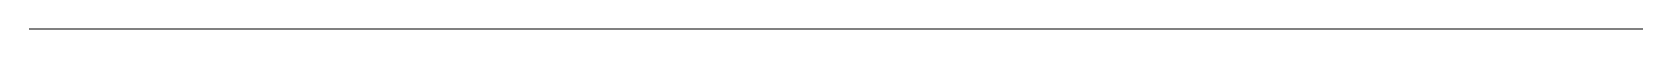
\begin{tikzpicture}
    \draw[gray,thick] (-6.5,0)--(14,0);
\end{tikzpicture}


 %%%%%%%%%%%%%%%%%%%%%%%% INICIO DEL CONTENIDO EN DOS COLUMNAS %%%%%%%%%%%%%%%%%%%%%
  
 \begin{multicols}{2}
   \begin{center}
         \LARGE{\textbf{Capítulo II, III: Vectores -  Estática}}\\	
         \vspace{0.2cm}
         % \Large {Lecturers Esteban Chalbaud \& Daniel Galviz} \\
         % \large{Teaching Assistant: Mauricio Gamonal \& Irvin Martínez}\\
         % \large{PhysicsLatam.com}\\
         % \vspace{0.2cm}
         \large{12 Agosto 2025, 5:59 pm (GMT-4)}\\
         % \vspace{0.2cm}
         \large{— Evaluación Parcial 2 —}
     \end{center}
    %%%%%%%%%%%%%%%%%%%%%%%%%%%%excercise%%%%%%%%%%%%%%%%%%%%%%%%%%%%%%%%%%%%%%%%
    \begin{excercise}[][][a) $d=12.29\ \mathrm{u}$; b)  $\alpha=12.11^\circ$]{ex:k28}{(\textbf{5 pts})
        Dados los puntos  $P(7,-2,5)$, $Q(-3,5,8 )$ y el vector $\vec{v}=\vec{\imath}+4\vec{\jmath}-4\vec{k}$:
        \begin{itemize}
            \item[a)] Encontrar la distancia del punto Q a la recta que pasa por P y es paralela al vector $\vec{v}$
            \item[b)] Calcular el ángulo formado por los vectores $\vec{QP}$ y la distancia del punto Q a la recta paralela a $\vec{v}$ del item a)
            \item[c)] Graficar correctamente todos los elementos del problema 
        \end{itemize}
         }
    \end{excercise}
    %%%%%%%%%%%%%%%%%%%%%%%%%%%%excercise%%%%%%%%%%%%%%%%%%%%%%%%%%%%%%%%%%%%%%%%
    \begin{excercise}[][][a) $\sum \vec{F}_i=\vec{0}$; b)  $\sum\tau_i=12\sqrt{5}\vec{\imath}+(6\sqrt{5}-20)\vec{k}$,  c) $\alpha=13.79 ^\circ\, \beta=90^\circ\, \gamma=103,79^\circ$;]{ex:k29}{(\textbf{5 pts})
         Se tiene dos pares de vectores fuerza que actúan en las aristas de la figura:
         \begin{figure}[H]
             \includegraphics[width=0.8\linewidth]{img/01_physics-i/03_statics/25_ex.png}
         \end{figure}
        la norma de cada par de  fuerzas opuestas son $F_1=F_2=10$ N, mientras $F_3=F_4=10$ N 
         \begin{itemize}
             \item[a)] Calcular los vectores fuerza, a partir de ello demostrar que la resultante es el vector nulo
             \item[b)] Calcular el torque resultante
             \item[c)] Encontrar los ángulos $\alpha, \beta, \gamma$ que forma el vector torque con cada uno de los ejes x, y, z, y  graficar
         \end{itemize}
         }
    \end{excercise}

    \begin{excercise}[][][$d=2.6\,\mathrm{m}$]{ex:11}{ (\textbf{1.5 pts})  
    Dos fuerzas paralelas, del mismo sentido, tienen magnitudes de $25\ \mathrm{N}$ y $40\ \mathrm{N}$.  
    La distancia de la línea de acción de la resultante a la fuerza mayor es de $1.0\ \mathrm{m}$.  
    Encontrar la distancia entre las fuerzas.  
    }
    \end{excercise}

    %%%%%%%%%%%%%%%%%%%%%%%%%%%%excercise%%%%%%%%%%%%%%%%%%%%%%%%%%%%%%%%%%%%%%%%
    \begin{excercise}[][][a) $F_1= 2.32\, \mathrm{kgf}  , F_2=25\, \mathrm{kgf}$; b)  $T=17.7\ \mathrm{kgf}$]{ex:k30}{(\textbf{5.5 pts})
        EL poste QE de longitud $10$ m es sujeto por el cable QP de modo que este no se resbale. El peso del poste es de $w=20$ kgf, $F_1$ y $F_2$ son fuerzas de reacción (normales a la superficie de la barra). 
        \begin{figure}[H]
             \centering
             \includegraphics[width=0.7\linewidth]{img/01_physics-i/03_statics/26_ex.png}
         \end{figure} 
         Considerar que todas las superficies son lisas (no hay fuerzas de fricción) y que el peso actua siempre del centro geométrico de la barra. 
        \begin{itemize}
             \item[a)] Calcular las reacciones $F_1$ y $F_2$ 
             \item[b)] Calcular la tensión $T$ del cable QP
             \item[c)] Resolver el problema usando el método vectorial y escalar para la segunda condición de quilibrio.
         \end{itemize} 
         }
    \end{excercise}
    %%%%%%%%%%%%%%%%%%%%%%%%%%%%excercise%%%%%%%%%%%%%%%%%%%%%%%%%%%%%%%%%%%%%%%%
    \begin{excercise}[img/01_physics-i/03_statics/14.png][0.7\linewidth][$T=125.2 \ \mathrm{N} $, $R=75.4\ \mathrm{N}$]{ex:25}{(\textbf{1.5 pts})
        Una esfera de peso $W=100$ N se sostiene mediante una cuerda AB (Fig.) y presiona una pared vertical lisa AC. Si $\alpha=37^\circ$ es el ángulo entre la cuerda y la pared, determinar la tensión en la cuerda y la reacción de la pared sobre la esfera.  
        } 
     \end{excercise}

    %%%%%%%%%%%%%%%%%%%%%%%%%%%%excercise%%%%%%%%%%%%%%%%%%%%%%%%%%%%%%%%%%%%%%%%
     \begin{excercise}[][][$\theta=53^\circ $, $T=500\ \mathrm{lbf}$]{ex:19}{(\textbf{1.5 pts})
        Para la Fig. Calcular el ángulo y la tensión en la cuerda AB si $M_1=300$ lbf y $M_2=400$ lbf.     
         \begin{figure}[H]
             \centering
             \includegraphics[width=0.4\linewidth]{img/01_physics-i/03_statics/12.png}
         \end{figure}
    } 
     \end{excercise}

\end{multicols}
